% Analítica Predictiva y Prescriptiva · TIC-60286 · Semana 8
% Contar la historia
% Compilar: pdflatex week-08.tex (dos veces)
%
% Plan de los 90 minutos (cierre de 20 minutos)
%   0–5    Dónde vamos y la parada 1, en el chat (láminas 2–3)
%   5–20   El paper: Dalal, Fowlkes y Hoadley (1989), el Challenger (láminas 5–9)
%  20–65   La aplicación (láminas 11–21): antes y después, con la cuenta a mano del beneficio neto
%          de B (4 min); la estructura con el expediente
%          de Latitud y una línea del chat reescrita en vivo (6); el título que dice el hallazgo,
%          cuatro parejas de figuras (12, tres por pareja); Knaflic (3); Sosa Escudero (2);
%          el error sembrado (5) y su traducción (4); las cinco preguntas y la parada 2 (9)
%  65–70   Puente: el task 8 y la logística de la sesión 9 (láminas 23–24)
%  70–90   Cierre: ensayo con jurado sobre el task 7 que trajeron (lámina 25): dos equipos,
%          tres minutos de presentación y tres de preguntas cada uno (12); la sala califica con
%          la rúbrica en una encuesta (3); qué recomendaciones sobrevivieron al choque (5)
%
% Variante con cierre de 30 minutos (decisión abierta: el ensayo con jurado los necesita)
%   0–5 y 5–20 no cambian.
%  20–55   La aplicación en 35 minutos: antes y después (3); la estructura (5); las cuatro parejas
%          a dos minutos cada una (8), o solo la de zonas y la de robustez a cuatro; Knaflic y
%          Sosa Escudero juntas (4); el error sembrado (4) y su traducción (3); las cinco preguntas
%          (4) y la parada 2 (4), que también puede pasar al ensayo como primera pregunta del jurado
%  55–60   El task 8 y la sesión 9
%  60–90   Ensayo con jurado: tres equipos, cuatro minutos de presentación y cuatro de preguntas
%          cada uno (24); la encuesta (2); el choque (4). En la lámina 25 cambian "dos equipos",
%          "tres minutos" y los tiempos entre paréntesis.
%
% De dónde salen las cifras y las figuras
%   Todas las cifras están en input/cifras_derivadas_week08.txt (las escribe input/_figuras_week08.R
%   y las rehace input/_verificacion_week08.R). Las del Challenger se calculan con los 23 vuelos de
%   input/challenger_orings.csv (la tabla 1 del artículo); la probabilidad de daño es una
%   reestimación (logística binaria), no una cifra del artículo. Las dos cifras del artículo
%   (0.13 y 0.02, de su resumen) están anotadas en el mismo archivo con su procedencia.
%   Que la noche anterior se compararon solo los vuelos con daño lo dice el informe de la Comisión
%   Rogers (1986, vol. 1, cap. VI). Ese informe cuenta veinte vuelos a 66 °F o más; la tabla del
%   artículo, que es la que usan las láminas, tiene diecinueve (23 vuelos en total).
%   Las cifras del curso son las selladas de las semanas 3 a 7 (datasets/aperturas/ y
%   datasets/week-07/cifras_week07.txt). La lámina del error sembrado usa las líneas error_sembrado*.
%   Las once figuras de figures/ las genera input/_figuras_week08.R.
% Esta semana no hay sobre sellado.

\documentclass{beamer}
\input{../../_beamer/preambulo_app.tex}
\semana{8}{Contar la historia}

\begin{document}

%%=================================================
%% Primer slide
\begin{frame}
\titlepage
\end{frame}

%% ====================================================== 0. DÓNDE VAMOS (0–5)
\begin{frame}{Dónde vamos}
\begin{columns}[T]
\begin{column}{0.48\textwidth}
\textbf{La semana pasada:} los escenarios. La tabla de supuestos, el VPN de las cuatro alternativas, la tabla de robustez y una recomendación con disparadores (el task 7). Hoy se ensaya ante un jurado, en el cierre.

\medskip
\textbf{Hoy, la pieza 8 del expediente:} la historia. El memo de una página para la junta de Latitud, tres láminas con títulos que dicen el hallazgo y la validación con un experto.
\end{column}
\begin{column}{0.52\textwidth}
\begin{block}{La sesión}
\small
\begin{enumerate}
  \item El paper: el Challenger y el gráfico que no mostró lo que los datos decían.
  \item Una acción y una cifra: la misma recomendación, dicha dos veces.
  \item El título que dice el hallazgo: cuatro figuras del curso, antes y después.
  \item Qué mostrar de un modelo, con un error sembrado.
  \item Las cinco preguntas de la junta.
  \item Cierre: ensayo con jurado (task 7).
\end{enumerate}
\end{block}
\end{column}
\end{columns}
\end{frame}

\begin{frame}{Antes de empezar}
\parada{chat}{En \textbf{una línea}: ¿qué le recomiendan a la junta de Latitud? Leemos cinco en voz alta.}
\medskip
\small Guarden su línea. Antes de terminar la sesión la van a reescribir con tres piezas: un verbo, una cifra en la moneda de la decisión y un riesgo.
\end{frame}

\seccion{El paper: el gráfico que no mostró lo que los datos decían}
%% ====================================================== 1. EL PAPER (5–20)
\begin{frame}{El Challenger: ¿anticipaban los datos la falla?}{Dalal, Fowlkes y Hoadley (1989), \emph{Journal of the American Statistical Association}}
\small
\begin{columns}[T]
\begin{column}{0.5\textwidth}
\textbf{Qué investigaron.} Si los datos disponibles antes del lanzamiento del Challenger (28 de enero de 1986) anticipaban la falla de los anillos que sellan las juntas de los cohetes cuando hace frío.

\medskip
\textbf{El contexto.} La temperatura prevista para el lanzamiento era \textbf{31\,°F}. Ningún vuelo anterior había despegado por debajo de \textbf{53\,°F}. La noche anterior, las reuniones entre la NASA y el fabricante de los cohetes le dieron poca consideración a la historia de daños según la temperatura (Comisión Rogers, 1986).
\end{column}
\begin{column}{0.5\textwidth}
\textbf{Qué datos y cómo.}
\begin{itemize}\itemsep3pt
  \item Los \textbf{23 vuelos anteriores} con datos de los anillos.
  \item De cada vuelo, la \textbf{temperatura} de la junta al lanzar y el número de \textbf{anillos con daño} (de seis).
  \item Una \textbf{regresión logística}: la probabilidad de daño en función de la temperatura.
  \item La pregunta de fondo: ¿qué decían esos 23 vuelos sobre un lanzamiento 22\,°F más frío que el más frío de todos?
\end{itemize}
\end{column}
\end{columns}
\end{frame}

\begin{frame}{Qué encontraron (1 de 3)}{La noche anterior se compararon solo los vuelos con daño}
\centering
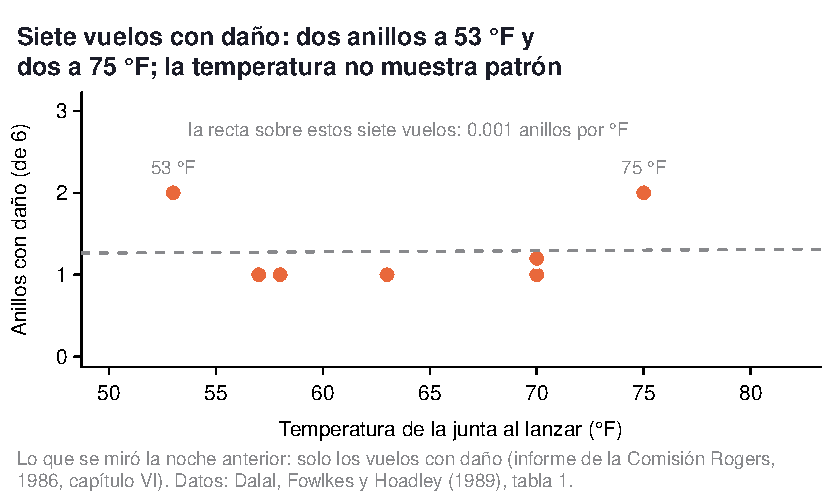
\includegraphics[width=0.86\textwidth]{figures/challenger_noche_anterior.pdf}

\raggedright\small
Siete vuelos con daño, entre 53 y 75\,°F. La recta sobre ellos es plana: 0.001 anillos por grado (correlación 0.02). \textbf{Con este gráfico, el frío no parece el problema.}
\end{frame}

\begin{frame}{Qué encontraron (2 de 3)}{Con los 23 vuelos, la relación con la temperatura es clara}
\centering
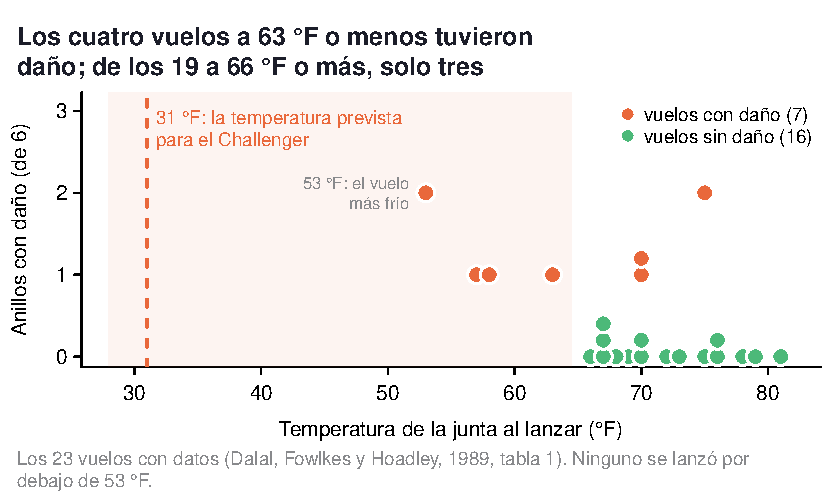
\includegraphics[width=0.86\textwidth]{figures/challenger_todos.pdf}

\raggedright\small
Faltaban los \textbf{16 vuelos sin daño}: todos despegaron a 66\,°F o más. Con los 23 vuelos, la correlación entre temperatura y daño es $-0.51$.
\end{frame}

\begin{frame}{Qué encontraron (3 de 3)}{La probabilidad de daño sube cuando la temperatura baja}
\centering
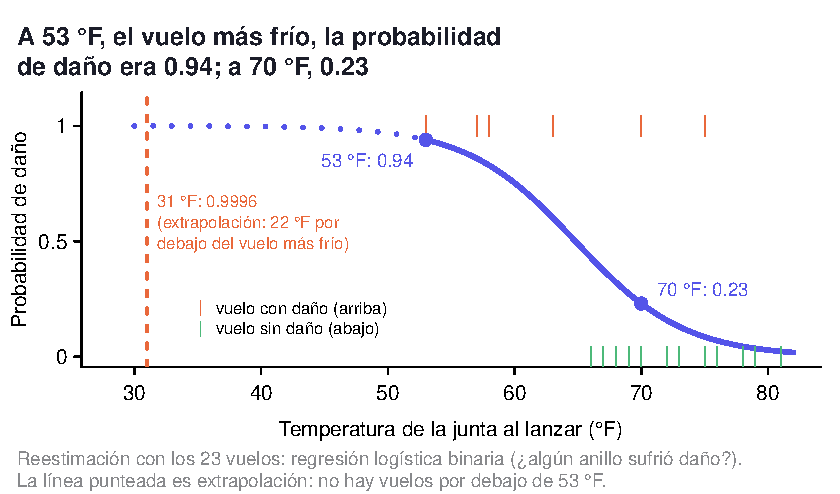
\includegraphics[width=0.83\textwidth]{figures/challenger_probabilidad.pdf}

\raggedright\footnotesize
\textbf{Reestimación con la tabla del artículo:} 0.94 a 53\,°F y 0.23 a 70\,°F. A 31\,°F el modelo dice 0.9996, y es una extrapolación. \textbf{El artículo} estima la probabilidad de una falla catastrófica a 31\,°F en al menos 0.13; a 60\,°F, en cerca de 0.02.
\end{frame}

\begin{frame}{Por qué importa para quien decide}
\begin{block}{Tres lecciones}
\begin{enumerate}\itemsep4pt
  \item \textbf{Cómo se presenta la evidencia decide.} Los mismos datos, dos gráficos, dos lecturas opuestas del riesgo.
  \item \textbf{Lo que se deja fuera del gráfico también es evidencia.} Los vuelos sin daño eran parte de la historia; en el estudio de aperturas, lo son los puntos de venta que siguen abiertos.
  \item \textbf{Fuera del rango de los datos, el modelo responde igual.} 31\,°F frente a un mínimo de 53; Barranquilla frente a seis ciudades. La extrapolación se dice.
\end{enumerate}
\end{block}
\parada{el puente}{La junta de Latitud no lee el expediente: ve una lámina. Si el gráfico no dice el hallazgo, la junta decide sin él.}
\end{frame}

\seccion{La aplicación: una acción y una cifra}
%% ====================================================== 2. LA APLICACIÓN (20–65)
\begin{frame}{Antes y después: la misma recomendación, dicha dos veces}
\begin{columns}[T]
\begin{column}{0.45\textwidth}
\begin{alertblock}{Antes}
``Probamos el modelo de la consultora B. \textbf{Tiene 80\,\% de exactitud} en validación. Recomendamos avanzar.''
\end{alertblock}
\footnotesize Es cierto (0.792). También lo es que la regla ``nadie cierra'' tiene 0.800 en el mismo lote y no encuentra un solo cierre.
\end{column}
\begin{column}{0.55\textwidth}
\begin{exampleblock}{Después}
``\textbf{Contratar a la consultora B.} Encuentra 12 de los 24 cierres del lote; evaluar a fondo su lista cuesta \peso 300 millones y evita pérdidas por \peso 1.500: \textbf{\peso 1.200 millones netos}.''
\end{exampleblock}
\footnotesize \textbf{La cuenta, a mano:} 25 avisos $\times$ 12 = 300 de costo; 12 cierres $\times$ 0.5 $\times$ 250 = 1.500 de pérdidas evitadas; 1.500 $-$ 300 = 1.200.
\end{column}
\end{columns}
\medskip
\importa{Un verbo, una cifra en la moneda de la decisión y el riesgo, en la frase siguiente: si la evaluación evita una de cada cuatro aperturas fallidas y no una de cada dos, gana A (469 frente a 450).}
\end{frame}

\begin{frame}{La estructura: situación, complicación, pregunta, respuesta}{El expediente de Latitud, puesto en orden}
\footnotesize
\begin{tabular}{@{}L{0.16\textwidth}L{0.54\textwidth}L{0.2\textwidth}@{}}
\toprule
Parte & Qué dice el memo de Latitud & Sale de la semana \\
\midrule
\textbf{Situación} & 46 tiendas, el Club con 3.908 suscriptores, \peso 1.000 millones para crecer y cuatro alternativas (A, B, C y D). & 1: la ficha \\
\textbf{Complicación} & El arriendo pedido en el norte de Barranquilla subió 18\,\% en 2026, y ningún punto de venta del estudio está allí: lo que se sabe de la tienda es extrapolación. & 2: la vigilancia; 5 y 6: los modelos \\
\textbf{Pregunta} & ¿En qué se invierten los \peso 1.000 millones este año? & 1: la ficha \\
\textbf{Respuesta} & Acelerar el Club con dos tramos: 212 millones de VPN en el escenario base; su peor caso pierde 71, frente a 271 de la tienda. Con el supuesto que manda y el disparador. & 7: los escenarios y la recomendación \\
\bottomrule
\end{tabular}

\smallskip
\textbf{La regla de la primera frase.} La respuesta abre con la acción; sigue la cifra; después, el riesgo. \textbf{En vivo:} reescribimos así una de las cinco líneas del chat. Otro expediente puede recomendar otra alternativa y vale lo mismo, si está igual de sustentado.
\end{frame}

\begin{frame}{El título que dice el hallazgo (1 de 4)}{La tasa de cierre por zona, semana 3}
\begin{columns}[T]
\begin{column}{0.4\textwidth}
{\footnotesize\textcolor{naranjaosc}{\textbf{Antes}}}\\[1pt]
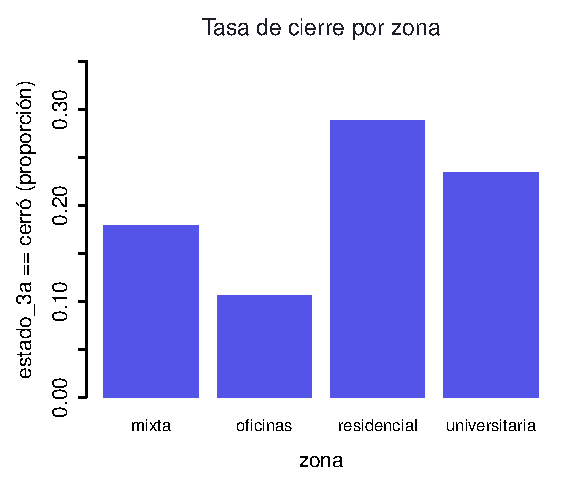
\includegraphics[width=\textwidth]{figures/zona_mala.pdf}

{\footnotesize ``Tasa de cierre por zona'' describe la variable. Quien lee solo el título no sabe qué pasó.\par}
\end{column}
\begin{column}{0.56\textwidth}
{\footnotesize\textcolor{verdeosc}{\textbf{Después}}}\\[1pt]
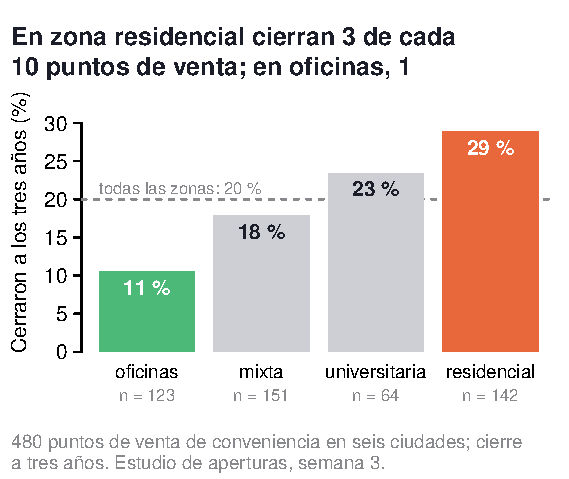
\includegraphics[width=\textwidth]{figures/zona_buena.pdf}
\end{column}
\end{columns}
\smallskip
{\footnotesize \textbf{Qué cambió:} el orden (de menor a mayor), el color (solo los dos extremos), la referencia (20\,\%) y el título, que dice quién, cuánto y frente a qué.\par}
\end{frame}

\begin{frame}{El título que dice el hallazgo (2 de 4)}{La tabla del líder, semana 4}
\begin{columns}[T]
\begin{column}{0.4\textwidth}
{\footnotesize\textcolor{naranjaosc}{\textbf{Antes}}}\\[1pt]
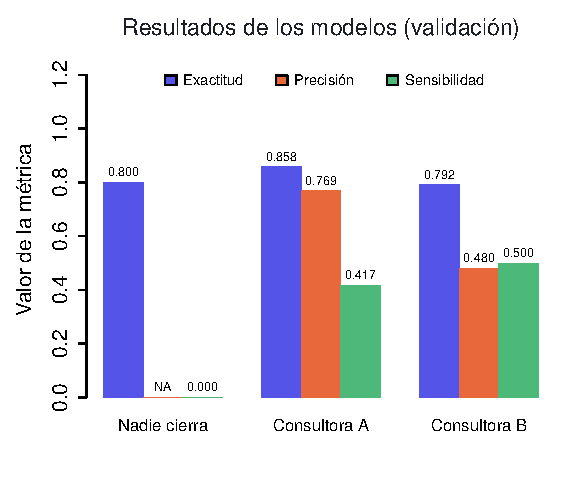
\includegraphics[width=\textwidth]{figures/lider_mala.pdf}

{\footnotesize Nueve métricas sin traducir. En exactitud, ``nadie cierra'' (0.800) parece empatar con las consultoras.\par}
\end{column}
\begin{column}{0.56\textwidth}
{\footnotesize\textcolor{verdeosc}{\textbf{Después}}}\\[1pt]
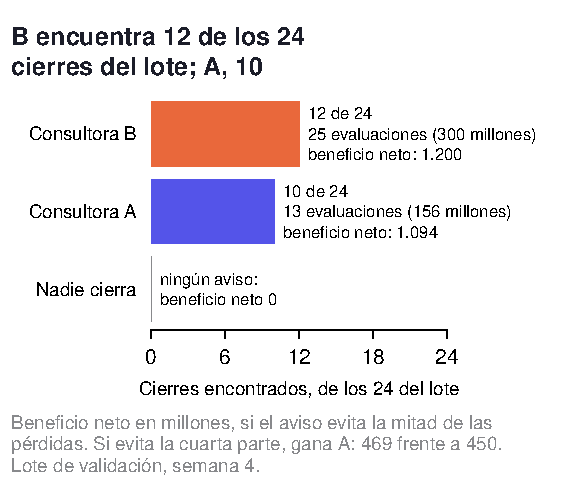
\includegraphics[width=\textwidth]{figures/lider_buena.pdf}
\end{column}
\end{columns}
\smallskip
{\footnotesize \textbf{Qué cambió:} la moneda. Cierres encontrados, evaluaciones y pesos en lugar de exactitud, precisión y sensibilidad. El giro de la efectividad va en la nota.\par}
\end{frame}

\begin{frame}{El título que dice el hallazgo (3 de 4)}{Las ventas base de los tres locales, semana 6}
\begin{columns}[T]
\begin{column}{0.4\textwidth}
{\footnotesize\textcolor{naranjaosc}{\textbf{Antes}}}\\[1pt]
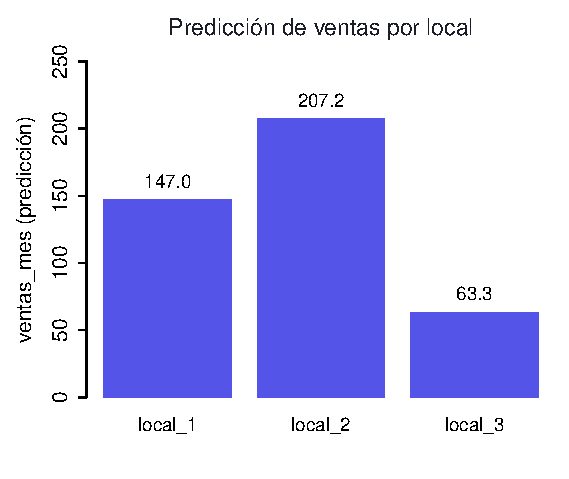
\includegraphics[width=\textwidth]{figures/bandas_mala.pdf}

{\footnotesize Tres puntos con un decimal: un pronóstico presentado como promesa, y Barranquilla sin asterisco.\par}
\end{column}
\begin{column}{0.56\textwidth}
{\footnotesize\textcolor{verdeosc}{\textbf{Después}}}\\[1pt]
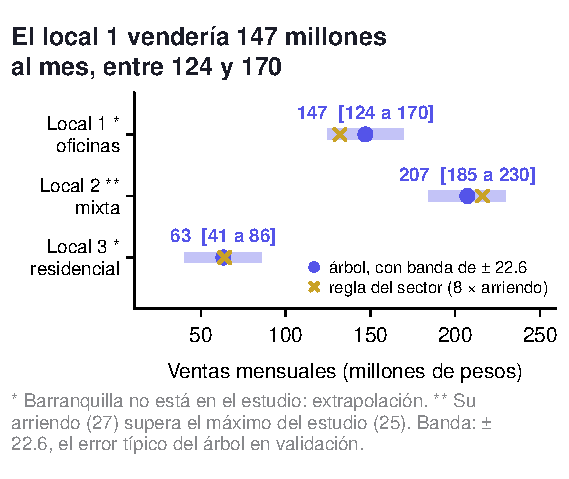
\includegraphics[width=0.97\textwidth]{figures/bandas_buena.pdf}
\end{column}
\end{columns}
\smallskip
{\footnotesize \textbf{Qué cambió:} el condicional (``vendería''), la banda de $\pm$ 22.6 millones al mes (cerca de \peso 204 millones de VPN) y los asteriscos de la extrapolación.\par}
\end{frame}

\begin{frame}{El título que dice el hallazgo (4 de 4)}{La tabla de robustez, semana 7}
\begin{columns}[T]
\begin{column}{0.4\textwidth}
{\footnotesize\textcolor{naranjaosc}{\textbf{Antes}}}\\[1pt]
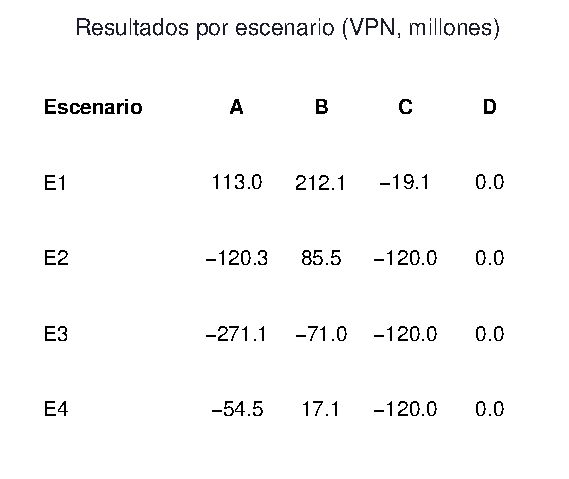
\includegraphics[width=\textwidth]{figures/robustez_mala.pdf}

{\footnotesize Dieciséis números correctos y ninguna lectura: ¿quién gana y dónde?\par}
\end{column}
\begin{column}{0.56\textwidth}
{\footnotesize\textcolor{verdeosc}{\textbf{Después}}}\\[1pt]
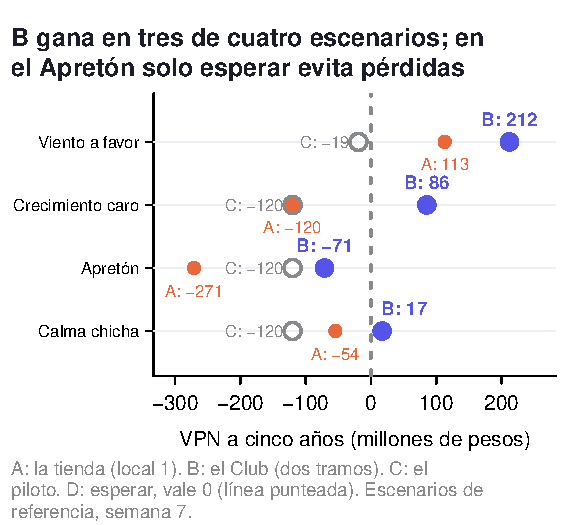
\includegraphics[width=0.86\textwidth]{figures/robustez_buena.pdf}
\end{column}
\end{columns}
\smallskip
{\footnotesize \textbf{Qué cambió:} los escenarios tienen nombre, el cero está marcado y B resalta. El arrepentimiento máximo (71 para B, 271 para A) se dice en voz alta.\par}
\end{frame}

\begin{frame}{Knaflic (2015): tres ideas para cada lámina}{\emph{Storytelling with Data}}
\begin{columns}[T]
\begin{column}{0.58\textwidth}
\begin{enumerate}\itemsep6pt
  \item \textbf{Contexto.} Antes de abrir el programa: ¿quién decide?, ¿qué necesita saber?, ¿qué debe hacer después de ver la lámina? Para Latitud: la junta, una acción y una cifra.
  \item \textbf{Quitar.} Todo lo que no ayuda a leer el hallazgo sobra: bordes, cuadrículas, decimales, leyendas que obligan a ir y volver, nombres de columnas.
  \item \textbf{Enfocar.} El color, el tamaño y la posición se gastan en una sola cosa: lo que la junta debe mirar. Lo demás va en gris.
\end{enumerate}
\end{column}
\begin{column}{0.42\textwidth}
\begin{block}{En las cuatro figuras}
\footnotesize
\textbf{Contexto:} el título dice quién, cuánto y frente a qué.

\smallskip
\textbf{Quitar:} los tres decimales, \texttt{estado\_3a}, la leyenda de tres métricas.

\smallskip
\textbf{Enfocar:} dos barras de color; B en morado; la banda y no el punto.
\end{block}
\end{column}
\end{columns}
\end{frame}

\begin{frame}{Sosa Escudero: los datos no hablan solos}
\begin{columns}[T]
\begin{column}{0.56\textwidth}
\begin{itemize}\itemsep6pt
  \item Una idea que recorre sus libros: \textbf{los datos no hablan solos}. Alguien eligió qué medir, con qué comparar y qué mostrar.
  \item En el Challenger, los datos eran los mismos la noche anterior y tres años después. Cambió la pregunta que se les hizo.
  \item En el expediente pasa igual: la tabla del líder no dice ``contraten a B''. Lo dice el equipo, con la hoja de costos al lado.
\end{itemize}
\end{column}
\begin{column}{0.44\textwidth}
\importa{Quien arma la lámina no es un mensajero neutral: responde por lo que la junta entiende. Por eso el memo dice también lo que no se sabe.}
\medskip
\footnotesize Lectura opcional de la semana: un ensayo, a elección, de \emph{Borges, big data y yo} (2022).
\end{column}
\end{columns}
\end{frame}

\begin{frame}{Resultados del modelo}{La lámina de un equipo para la junta}
\begin{columns}[T]
\begin{column}{0.52\textwidth}
\scriptsize
\textbf{Tabla cp (rpart, xval = 10)}\\[2pt]
{\ttfamily\setlength{\tabcolsep}{3.5pt}
\begin{tabular}{@{}rrrrr@{}}
\toprule
CP & nsplit & rel error & xerror & xstd \\
\midrule
0.04861 & 0 & 1.000 & 1.000 & 0.105 \\
0.03125 & 6 & 0.639 & 1.028 & 0.106 \\
0.02778 & 10 & 0.514 & 1.000 & 0.105 \\
0.01389 & 16 & 0.347 & 1.111 & 0.110 \\
\bottomrule
\end{tabular}}

\medskip
\textbf{Impureza de Gini (árbol de dos niveles)}\\[2pt]
{\ttfamily raíz 0.320\\ hojas 0.111 / 0.354 / 0.219 / 0.496}
\end{column}
\begin{column}{0.46\textwidth}
\scriptsize
\textbf{Matriz de confusión (validación)}\\[2pt]
{\ttfamily
\begin{tabular}{@{}lrr@{}}
\toprule
 & obs = 1 & obs = 0 \\
\midrule
pred = 1 & 15 & 11 \\
pred = 0 & 9 & 85 \\
\bottomrule
\end{tabular}}

\medskip
\textbf{Métricas}\\[2pt]
{\ttfamily accuracy 0.819 (train), 0.833 (test)\\
AUC 0.765 (A: 0.845; B: 0.786)}
\end{column}
\end{columns}
\medskip
\parada{error sembrado}{Todo es correcto y todo sale del expediente. ¿Qué entiende la junta? ¿Qué puede decidir distinto después de ver esta lámina? Dos minutos en parejas.}
\end{frame}

\begin{frame}{La misma evidencia, traducida}{Qué mostrar de un modelo y qué no}
\footnotesize
\begin{tabular}{@{}L{0.57\textwidth}L{0.34\textwidth}@{}}
\toprule
Se muestra & Queda en el anexo \\
\midrule
\textbf{Las reglas, como política.} Con menos de 165 peatones por hora y un operador con menos de 9 años, cierran 5 de cada 10 (75 puntos de venta). & El dibujo con nodo, corte y cp; la tabla de poda. \\
\textbf{La matriz, en avisos.} De 26 avisos del árbol, 15 son cierres reales; se escapan 9 de los 24. & 15, 11, 9 y 85, sin nombre. \\
\textbf{El error, en pesos.} El árbol de ventas se equivoca en 22.6 millones al mes por punto de venta: cerca de \peso 204 millones de VPN. & Gini 0.320; AUC 0.765. \\
\textbf{Lo que el modelo no vio.} Ningún punto de venta del estudio está en Barranquilla; el arriendo del local 2 (27) supera el máximo del estudio (25). & La exactitud de entrenamiento (0.819). \\
\bottomrule
\end{tabular}

\smallskip
\importa{La prueba de cada cifra: ¿la junta puede hacer algo distinto si la conoce? Con ``cierran 5 de cada 10'' evalúa a fondo ese perfil. Con ``Gini 0.496'' no puede hacer nada.}
\end{frame}

\begin{frame}{Las cinco preguntas de la junta}
\begin{columns}[T]
\begin{column}{0.46\textwidth}
\begin{enumerate}\itemsep4pt
  \item ¿Qué dato cambiaría su recomendación?
  \item ¿Qué pasa en el escenario adverso?
  \item ¿Por qué no esperar?
  \item ¿Qué no saben?
  \item ¿Qué medirían primero?
\end{enumerate}
\medskip
{\footnotesize En la sesión 9, las dos primeras van para todos los equipos; la tercera es libre. Se responde en dos líneas y con una cifra del expediente.\par}
\end{column}
\begin{column}{0.54\textwidth}
{\footnotesize
\textbf{¿Qué pasa en el escenario adverso?}

\smallskip
\textcolor{naranjaosc}{\textbf{Mal:}} ``Es poco probable que ocurra.''

\smallskip
\textcolor{verdeosc}{\textbf{Bien:}} ``En el Apretón, B pierde 71 millones y A, 271. Por eso el segundo tramo del Club se condiciona a lo que traiga el primero.''\par}

\medskip
\parada{chat}{Un equipo al azar responde: ¿qué dato cambiaría su recomendación? Con una cifra.}
\end{column}
\end{columns}
\medskip
{\footnotesize \textbf{Con las cifras de referencia:} las ventas del local 1. Por debajo de 145.4 millones al mes, la tienda deja de crear valor; la predicción es 147.0, con una banda de 124.4 a 169.7.\par}
\end{frame}

\seccion{El task y el cierre}
%% ====================================================== 3. PUENTE (65–70)
\begin{frame}{Task 8: la historia para la junta}
\begin{columns}[T]
\begin{column}{0.55\textwidth}
\small
\textbf{Qué se entrega} (en equipo, antes de la sesión 9; 90 minutos más la entrevista; esta semana no hay sobre sellado):
\begin{itemize}\itemsep3pt
  \item el memo de una página: una acción y una cifra, con el riesgo, el supuesto que manda y el disparador (1.5);
  \item el esqueleto de tres láminas con títulos que dicen el hallazgo (1.0);
  \item la validación con el experto: quién, su rol, la fecha, tres reacciones textuales y qué cambió (1.5);
  \item las respuestas a las cinco preguntas, dos líneas cada una (0.5);
  \item el acta y la declaración de IA (0.5).
\end{itemize}
\end{column}
\begin{column}{0.45\textwidth}
\begin{exampleblock}{La entrevista: 20 minutos}
\footnotesize ¿Qué de estos escenarios le parece inverosímil? ¿Qué supuesto cambiaría? ¿Qué haría usted con los \peso 1.000 millones?
\end{exampleblock}
\begin{alertblock}{Lo que no cuenta}
\footnotesize Una cifra que no esté en el expediente. Un título que no sea un hallazgo. Una banda convertida en punto. Una entrevista sin nombre, rol y fecha. Jerga sin traducir.
\end{alertblock}
\end{column}
\end{columns}
\end{frame}

\begin{frame}{La sesión 9: la defensa ante la junta}
\begin{columns}[T]
\begin{column}{0.56\textwidth}
\small
\begin{itemize}\itemsep4pt
  \item \textbf{No hay clase ni cierre:} la sesión entera es la defensa.
  \item \textbf{El orden se sortea} al empezar.
  \item \textbf{Seis minutos de presentación}, con las tres láminas. \textbf{El expositor de cada lámina también se sortea:} cualquiera presenta cualquier parte.
  \item \textbf{Seis minutos de junta:} se abre la posición sellada de la semana 1 y se compara con la recomendación final; después, las preguntas.
  \item La sala califica con la rúbrica en una encuesta: es retroalimentación, no nota.
\end{itemize}
\end{column}
\begin{column}{0.44\textwidth}
\begin{block}{La rúbrica (35\,\% del curso)}
\footnotesize
Decisión y evidencia: 40\\
Supuestos y robustez: 25\\
La historia: 20\\
Respuesta a la junta: 15\\
Ajuste individual del expositor: $\pm$ 0.5
\end{block}
{\footnotesize \textbf{Después de la defensa:} el memo individual de transferencia (20\,\%), una página sobre una decisión de la organización de cada uno. La fecha se publica en Canvas.\par}
\end{column}
\end{columns}
\end{frame}

%% ====================================================== 4. CIERRE (70–90)
\begin{frame}{Cierre: ensayo con jurado (task 7)}
\begin{enumerate}\itemsep5pt
  \item \textbf{Dos equipos al azar} (12 minutos). Cada uno presenta su recomendación y sus disparadores en \textbf{tres minutos}. Siguen \textbf{tres minutos de preguntas} de la ``junta'': el profesor y dos voluntarios de otros equipos, con las cinco preguntas en la mano.
  \item \textbf{La sala califica con la rúbrica} en una encuesta (3 minutos): decisión y evidencia, supuestos y robustez, la historia, respuesta a la junta.
  \item \textbf{El choque} (5 minutos): arriendos 18\,\% más altos y tasa de 14\,\%. ¿Qué recomendaciones sobrevivieron? Con las cifras de referencia, B con dos tramos sigue primera (194.5); la tienda en el local 1 pasa de 14.6 a $-105.1$; el piloto queda en $-120.0$; esperar vale 0.
\end{enumerate}
\medskip
\importa{Lo que se ensaya hoy es lo que se califica en la sesión 9: una acción, una cifra, un riesgo y una respuesta con el expediente en la mano.}
\end{frame}

\begin{frame}{Referencias}
\small
\begin{itemize}\itemsep5pt
  \item Dalal, S. R., Fowlkes, E. B. y Hoadley, B. (1989). Risk analysis of the space shuttle: Pre-Challenger prediction of failure. \emph{Journal of the American Statistical Association}, 84(408), 945--957.
  \item Knaflic, C. N. (2015). \emph{Storytelling with Data: A Data Visualization Guide for Business Professionals}. Wiley.
  \item Presidential Commission on the Space Shuttle Challenger Accident (1986). \emph{Report to the President} (informe de la Comisión Rogers), vol. 1, cap. VI.
  \item Sosa Escudero, W. (2022). \emph{Borges, big data y yo}. Siglo XXI.
\end{itemize}
\end{frame}

\end{document}
